%%%%%%%%%%%%%%%%%%%%%%%%%%%%%%%%%%%%%%%%%%%%%%%%%%%%%%%%%%%%%%%%%%%%%%%%%%%%%%%%
\documentclass[twocolumn]{revtex4}

%%%%%%%%%%%%%%%%%%%%%%%%%%%%%%%%%%%%%%%%%%%%%%%%%%%%%%%%%%%%%%%%%%%%%%%%%%%%%%%%
% Note that comments begin with a "%" and are not turned into text in the .pdf
% document.
%%%%%%%%%%%%%%%%%%%%%%%%%%%%%%%%%%%%%%%%%%%%%%%%%%%%%%%%%%%%%%%%%%%%%%%%%%%%%%%%

%%%%%%%%%%%%%%%%%%%%%%%%%%%%%%%%%%%%%%%%%%%%%%%%%%%%%%%%%%%%%%%%%%%%%%%%%%%%%%%%
% Include some extra packages.
%%%%%%%%%%%%%%%%%%%%%%%%%%%%%%%%%%%%%%%%%%%%%%%%%%%%%%%%%%%%%%%%%%%%%%%%%%%%%%%%
\usepackage[]{graphicx}
%%%%%%%%%%%%%%%%%%%%%%%%%%%%%%%%%%%%%%%%%%%%%%%%%%%%%%%%%%%%%%%%%%%%%%%%%%%%%%%%

%%%%%%%%%%%%%%%%%%%%%%%%%%%%%%%%%%%%%%%%%%%%%%%%%%%%%%%%%%%%%%%%%%%%%%%%%%%%%%%%
\begin{document}

%%%%%%%%%%%%%%%%%%%%%%%%%%%%%%%%%%%%%%%%%%%%%%%%%%%%%%%%%%%%%%%%%%%%%%%%%%%%%%%%
\title{
Monte Carlo Methods to Predict the Weather}



\author{Jeff Petteys}
\affiliation{Siena College, Loudonville, NY}

\date{\today}

\begin{abstract}
    
For the final project in CSIS200, we were assigned questions that were to predict rainfall values/how many times it would rain in a given month with 30 days. Through the use of lists, loops, numpy and other tools from this course, we predicted the odds of it raining when certain days had assigned percentages (their probabilities). We did this both {\it analytically}, where the solution can be written by hand with a formula, and {\it numerically} using {\bf Monte Carlo} approaches. This is where we set up situations and generate random numbers multiple times to stimulate a situation; both ways are accurate.
\end{abstract}

\maketitle
%%%%%%%%%%%%%%%%%%%%%%%%%%%%%%%%%%%%%%%%%%%%%%%%%%%%%%%%%%%%%%%%%%%%%%%%%%%%%%%%

%%%%%%%%%%%%%%%%%%%%%%%%%%%%%%%%%%%%%%%%%%%%%%%%%%%%%%%%%%%%%%%%%%%%%%%%%%%%%%%%
\section{Introduction}
%%%%%%%%%%%%%%%%%%%%%%%%%%%%%%%%%%%%%%%%%%%%%%%%%%%%%%%%%%%%%%%%%%%%%%%%%%%%%%%%
Each question had a different goal with different probabilities assigned to each day. Through the use of NumPy, we we able to generate random numbers to represent probabilities. For example, if a question were to say that there's a two-percent chance of it raining on a given day, we would've generated a number between 0-1. If it were .01 or .02, we would conclude that it rains on that day. Any value .03 or higher means that it won't rain on that day. This idea was expressed throughout the problems.

%%%%%%%%%%%%%%%%%%%%%%%%%%%%%%%%%%%%%%%%%%%%%%%%%%%%%%%%%%%%%%%%%%%%%%%%%%%%%%%%
\section{Problem 1}
%%%%%%%%%%%%%%%%%%%%%%%%%%%%%%%%%%%%%%%%%%%%%%%%%%%%%%%%%%%%%%%%%%%%%%%%%%%%%%%%
For the first question, we were told that there's a 20 percent chance that it can rain on any day in a 30 day month. We were told to determine the odds of it raining on one day and one day {\bf only} in a month. I figured this out analytically by transforming the question into terms of probability (using and, or, etc.). I said that there's a 20 percent chance of it raining on one random day in a month only {\it and} there's an 80 percent chance of it not raining on the remaining 29 days. The equation looks as so: $ .2 * 1 * .8^{29} * 30 $. In other words, 20 percent times 1 day, multiplied by 80 percent 29 times (for the rest of the month) all multiplied by 30 days in the month.  This concludes that there's a .9284\% chance of it raining on one day and one day only in a given month.
\\For the Monte Carlo approach, I wanted to create a fucntion that would loop over random values to determine if it was raining on a given day. If the random value were to be between .2 and 1.0, it would mean that it doesn't rain. If the value were between 0 and .2, it would make it rain! I then wanted to create a list of all values between 0 and .2. If the length of the list was one, that means that there was only one day that month where it rained, (yay!) two or more values were in the list, that would mean it rained more than once in that month, which wasn't what we were looking for. I then used a larger setup where there were 1000, or any large number, rooms to see on a larger scale if the analytical and numerical numbers would be the same.


%%%%%%%%%%%%%%%

\section{Problem 2}

I took the same approach for question two, much like number one. This was asking for the odds of it raining 8 days or more in a month where there's a 10 percent chance that it will rain on any given day. I used the same function from the previous problem except changed 20 percent to 10 percent chance of it raining. I then changed the second function to see if the length of the list had 8 or more values. If it does, there's a statement that will appear saying there's at least 8 days in the given month where it rains. If it doesn't loop through, theres an else statement saying there were 7 days or less that it rained in that month. I did the same thing as problem one and set it up on a larger scale.
%%%%%%%%%%%%%%%

\section{Problem 3a}

This section wrote that the percentages were different for each centimeter of rainfall likliness. the chances of 1 cm is 20\%,  2 cm 30\%, 3 cm 30\%, 4 cm 10\%, and 5 cm 10\%. However, there are restraints depending if the previous number of days produced rain. The circumstances are as follows: 
If it is the first day of the month, there is a 10\% chance of rain.
If it rained 1 day before, but not 2 days before, there is a 20\% chance of rain.
If it rained both of the 2 days before, but not the 3rd day before, there is a 25\% chance of rain.
If it rained for the 3 days (or more) before, there is a 5\% chance of rain.
Otherwise, there is a 10\% chance of rain. I was unable to demonstrate the odds of there being at least 10 cm of rain in a given month, but my assumption of what the results would look like are stated in section 3b.


\subsection{3B}

This part is where I made up a list of values to show the distribution of expected rainfall on a histogram. At the beginning of question three, it said that on a certain day the odds of the daily rain fall were: 1 cm 20\%, 2 cm 30\%, 3 cm 30\%, 4 cm 10\%, and 5 cm 10\%. I then wanted to make a list where there were 200 values between 0-1, 300 between 1-2 and so on depending on the percent values. This would've created a right-skewed graph. However, I had to come up with my own data as I was unable to complete the previous part of this question.  Fig.~\ref{graph}.
\begin{figure}[!h]

\centering
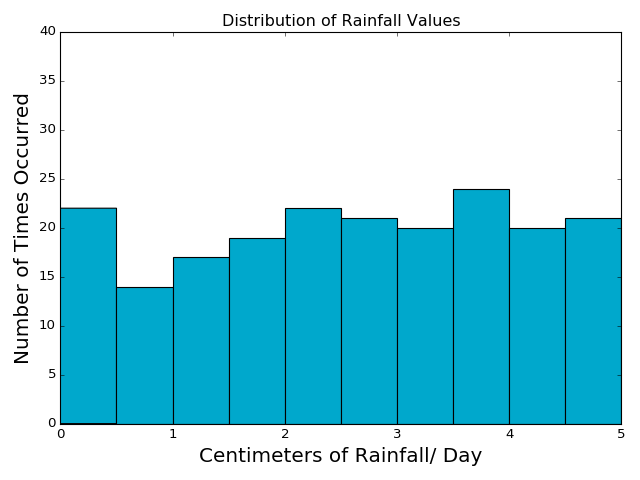
\includegraphics[width=0.5\textwidth]{graph.png}
\caption{My histogram! \label{graph}}


\end{figure}

\subsection{3C}


In this section I created a simple equation where it took the values and divided it by the total number, in this case 200 which gives us the average.

\subsection{3D}

In this section we looked at the uncertainty in our answers. One says "I'm 95\% confident that the correct values fall between two values". This method disregards the values on both ends to give a higher confidence level that the information in the middle is more accurate.
%%%%%%%%%%%%%%%%%%%%%%%%%%%%%%%%%%%%%%%%%%%%%%%%%%%%%%%%%%%%%%%%%%%%%%%%%%%%%%%%
\end{document}
%%%%%%%%%%%%%%%%%%%%%%%%%%%%%%%%%%%%%%%%%%%%%%%%%%%%%%%%%%%%%%%%%%%%%%%%%%%%%%%%
